	\chapter{Convolutional Neural Networks}
	\section{Frequently Asked Questions}

	\resetquestioncounter{}
	\begin{qanda}
		\begin{question}
 What is Computer Vision?
		\end{question}
		\begin{answer}
Computer Vision is a field of Artificial Intelligence that enables computers or systems to derive or extract meaningful information from a digital image or video data and take actions or recommendations based on this information.
		\end{answer}
	\end{qanda}

	\begin{qanda}
		\begin{question}
 What is the Normalization of pixels?
		\end{question}
		\begin{answer}
For most image data, the pixel values are integers with values between 0 and 255. Normalization scales these pixel values between 0 and 1 before modeling.
		\end{answer}
	\end{qanda}

	\begin{qanda}
		\begin{question}
Why should Normalization be performed on pixels?
		\end{question}
		\begin{answer}
Neural networks process inputs using small weight values and inputs with large integer values can disrupt or slow down the learning process, so it is a good practice to normalize the pixels so that the values would range between 0 and 1.
		\end{answer}
	\end{qanda}

	\begin{qanda}
		\begin{question}
How is smoothing performed on images?
		\end{question}
		\begin{answer}
Smoothing an image is required to reduce noise and blur the false edges. Smoothing is usually performed using Gaussian Blur. Gaussian filtering is highly effective at removing noise from the image. We can use the below code to perform Gaussian Blur.

		\begin{code}[\codenumbering]{}
			\codeitemnonumber blur\_image = cv2.GaussianBlur(original\_image, (5,5), 0)
		\end{code}
		\end{answer}
	\end{qanda}

	\begin{qanda}
		\begin{question}
Will the images always be provided in zip file format?
		\end{question}
		\begin{answer}
The image data sets are usually provided in the following formats:

	\begin{bulletedlist}
		\item {\bfseries Folders/Directories}: The whole data set can be given in a single directory or a zip file which can be extracted to get a directory. This directory can contain sub-folders like training and testing. The training and testing folders may contain individual sub-folders for each category of image. The whole structure can be observed in the \figurename~\ref{fig:cnnimagesinfiles}.
		\item {\bfseries TensorFlow data sets}: The data sets can be loaded from as shown in \figurename~\ref{fig:cnntensorflowdataset}.
		\item {\bfseries numpy arrays}: The images can also be given as numpy arrays and the labels to the corresponding images can be given in a CSV file.  The images that are converted into numpy arrays can be given in \textcode{images.npy} file and the labels corresponding to each image can be given in the \textcode{labels.csv file}.  The \textcode{np.load()} function can be used to read the numpy arrays and the \textcode{pd.read\_csv()} function from pandas can be used to read the \textcode{csv} file as shown in \figurename~\ref{fig:cnnnumpyarraydataset}.
	\end{bulletedlist}
		\end{answer}
	\end{qanda}

	\begin{figure}[h]
		\centering
		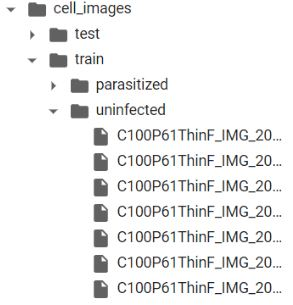
\includegraphics[height=2in]{cnnimagesinfiles}
		\caption[Cross validation]{Cross validation.}
		\label{fig:cnnimagesinfiles}
	\end{figure}

	\begin{figure}[h]
		\centering
		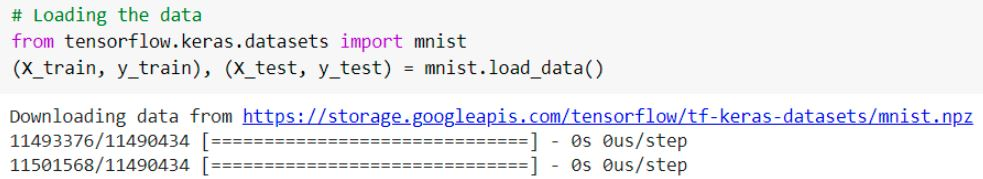
\includegraphics[width=\textwidth-1in]{cnntensorflowdataset}
		\caption[Loading a TensorFlow image data set]{Loading a TensorFlow image data set.}
		\label{fig:cnntensorflowdataset}
	\end{figure}

	\begin{figure}[h]
		\centering
		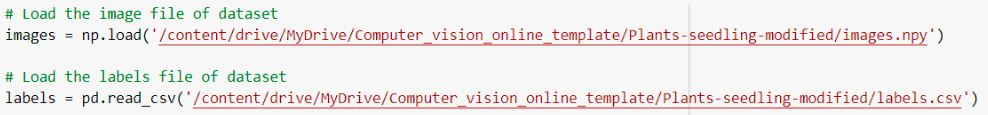
\includegraphics[width=\textwidth]{cnnnumpyarraydataset}
		\caption[Numpy array loading of image data set]{Numpy array loading of image data set.}
		\label{fig:cnnnumpyarraydataset}
	\end{figure}

	\begin{qanda}
		\begin{question}
Do we need to split the image data into train and test sets before pre-processing?
		\end{question}
		\begin{answer}
The splitting of image data should be performed before any operations or pre-processing steps on images.  One way is to divide the data set into two subsets:
	\begin{numberedlist}
		\item Training set: a subset to train a model.
		\item Test set: a subset to test the model.
	\end{numberedlist}

Separating the data enables you to evaluate your model generalization capabilities and have an idea of how it would perform on unseen data.  Good performance on the test set is a useful indicator of good performance on new data in general, assuming that:
	\begin{bulletedlist}
		\item The samples were drawn independently and at random from the distribution to create the test set.
		\item The test set is large enough.	
	\end{bulletedlist}

The second way is to divide the data set into three subsets:
	\begin{numberedlist}
		\item Training set: a subset to train a model.
		\item Validation set: a subset to validate and tune our model.
		\item Test set: a subset to test the model.
	\end{numberedlist}
		\end{answer}
	\end{qanda}

	\begin{qanda}
		\begin{question}
What is the difference between MNIST and Fashion MNIST data sets that are used in the course?
		\end{question}
		\begin{answer}
The MNIST data consists of images of 10 handwritten digits from 0 to 9, and this data set can be directly loaded using the \textcode{load\_data()} function of TensorFlow.  Whereas, Fashion MNIST can also be loaded using the same \textcode{load\_data()} function, it consists of fashion images like shoes, shirts, etc belonging to 10 different categories.
		\end{answer}
	\end{qanda}

	\begin{qanda}
		\begin{question}
What is the difference between \textcode{resize()} and \textcode{reshape()} functions (in context of images)?
		\end{question}
		\begin{answer}
The \textcode{reshape()} function changes the shape only and not the number of pixels.  For example, the image of size 6 x 4 can be reshaped into 12 x 2.  Here we did not change the number of pixels.  But an image of 6 x 6 can be resized into 10 x 10 using the resize function.  Here the number of pixels are increased.
		\end{answer}
	\end{qanda}

	\begin{qanda}
		\begin{question}
Which function can be used to get the names of labels that are encoded using an encoder?
		\end{question}
		\begin{answer}
The \textcode{inverse\_transform()} function can be used to decode the labels from the encoded vectors.  For example: if a label ``car'' is encoded using a label binarizer into an array of [0,0,1] then \textcode{inverse\_transform()} can be used to get the label name from this array.
		\end{answer}
	\end{qanda}

	\begin{qanda}
		\begin{question}
How to unzip a zipfile in Google Colab?
		\end{question}
		\begin{answer}
The unzip command can be used to unzip the file in Google Colab.
		\begin{code}[\codenumbering]{}
			\codeitemnonumber !unzip ``path to the file''
		\end{code}
		\end{answer}
	\end{qanda}

	\section{ANNs versus CNNs}
	\subsection{Image Classification Using ANNs}
	\subsubsection{Method}

	\begin{bulletedlist}
		\item If the images are RGB, we know that each image will have 3 channels, which will be represented by 3 matrices - each matrix numerically representing the pixel intensity values from that channel.
		\item The information about brightness, contrast, edges, shape, texture, shadows etc. of an image does not depend on color. So the RGB representation of images only adds to the complexity, and may be replaced by their gray scale version instead.
		\item For that reason, we will use the gray scale color space, which isolates the color information into a single channel.
		\item In ANNs, one neuron would be used for each input (\figurename~\ref{fig:imageprocessingwithann}). Here the inputs are the pixel values in an image.  For an image with 28 x 28 pixels, the flattened input layer will have 28*28 = 784 inputs.
		\item Every node/element in the output vector refers to an output class.  The input sample is labeled according to the class with the highest score.
	\end{bulletedlist}

	\begin{figure}[tbh]
		\centering
		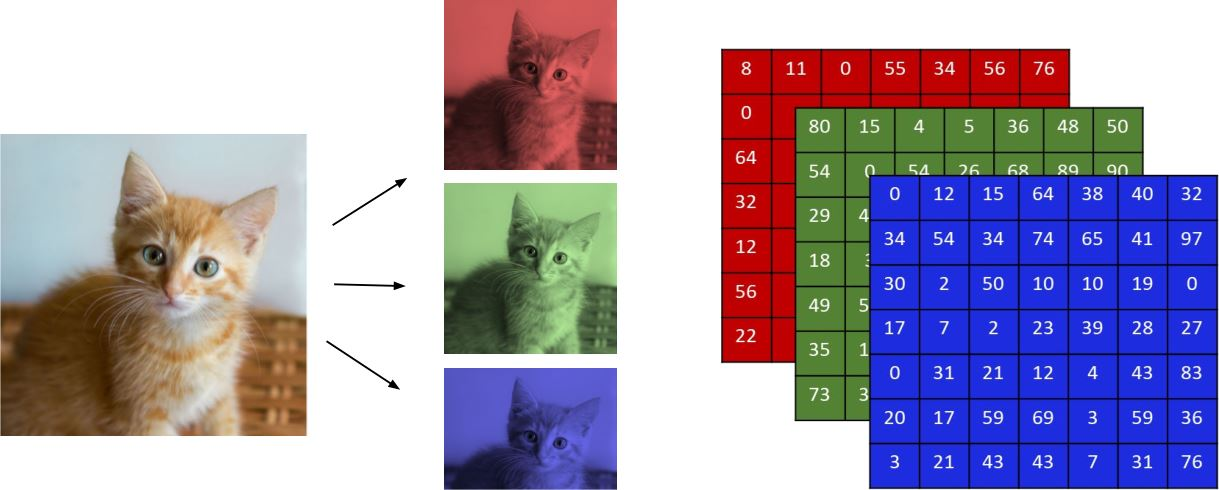
\includegraphics[height=1.5in]{catimagetorgbchannels}
		\caption[Image broken down into RGB channels]{Image broken down into RGB channels.}
		\label{fig:catimagetorgbchannels}
	\end{figure}

	\begin{figure}[tbh]
		\centering
		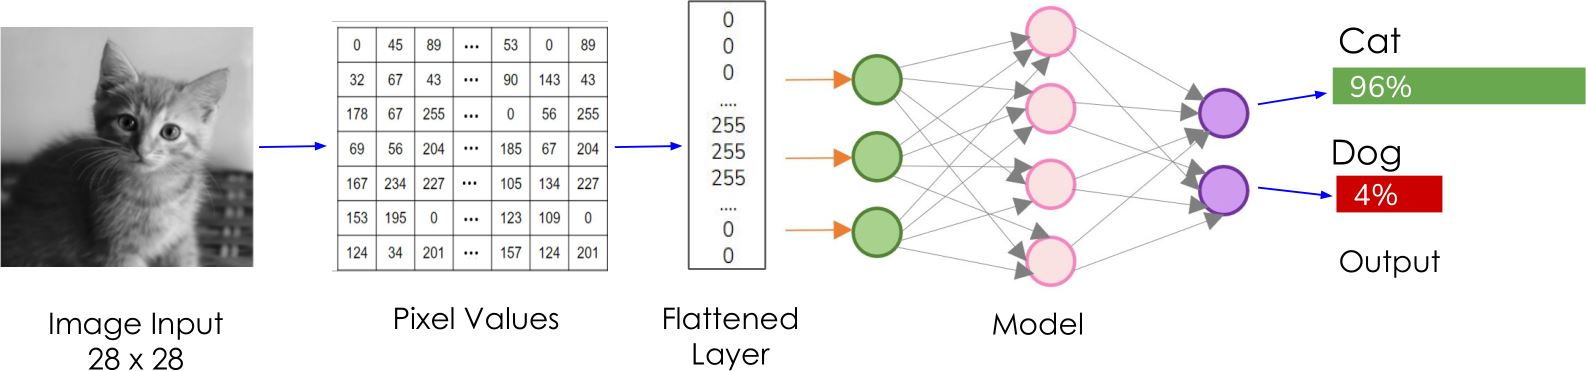
\includegraphics[width=\textwidth]{imageprocessingwithann}
		\caption[Image processing with ANNs]{Image processing with ANNs.}
		\label{fig:imageprocessingwithann}
	\end{figure}


	\subsubsection{Challenges with Image Classification Using ANNs}

	\begin{bulletedlist}
		\item One of the main disadvantages of ANNs is that \textbf{they are not translation invariant}.  For example, a cat may be present in the center, left, or right of an image.  ANNs would try to learn the location the cat is present as an indicator of its presence.  This may give inconsistent results.
		\item Another problem with ANNs is that \textbf{they lose spatial information} after getting the image matrix converted into a flattened array.  This means ANNs do not leverage the fact that nearby pixels are more strongly related than distant ones.
		\item Yet another disadvantage of ANNs for image classification, has to do with detecting which features of an image are important and which ones are not. When detecting the presence of the object, there is no use of looking at the background or other features of an image. There is unfortunately no scope to use this idea in a traditional ANN, which may give importance to every pixel in an
image, and will hence try to learn the background of the object as well.  For example, a cat remains a cat whether it is in the garden or on a table.  However, an ANN will wrongly learn about the background and assume that a cat appears in a specific background.
	\end{bulletedlist}


	\subsubsection{The Computationally Expensive Nature of ANNs}
	\begin{bulletedlist}
		\item ANNs are very computationally expensive.
		\item To use an ANN, we would first have to flatten the input. Using just two fully-connected layers (of 32 and 2 nodes each) on the input image of 28x28x1, we observe that there are already about 50,000 trainable parameters, and this would just increase with an increase in the number of layers.
	\end{bulletedlist}

	\begin{figure}[tbh]
		\centering
		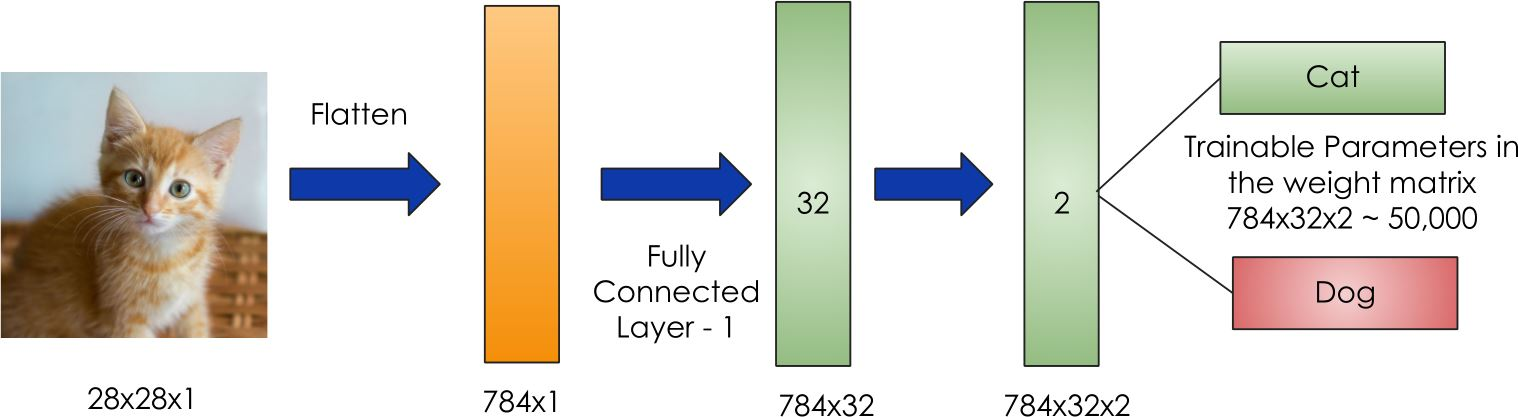
\includegraphics[width=\textwidth-1in]{fullyconnectannforimageprocessing}
		\caption[Expense of image processing with ANNs]{Expense of image processing with ANNs.}
		\label{fig:fullyconnectannforimageprocessing}
	\end{figure}

	\subsection{Spatial and Translational Invariance of CNNs}

	\begin{bulletedlist}
		\item CNNs have the in built property of handling positional shifts, or translations of a given image. They are
spatially and translationally invariant (see \figurename~\ref{fig:translationalinvarianceforcnns}).
		\item In the below example, we have three images of a cat.  It obviously remains a cat regardless of whether it appears in the left, the center or the top right corner of the image.  Unlike ANNs, CNNs are able to understand this, as you would expect for any practical computer vision model.
		\item CNNs achieve this through the use of convolutional and pooling layers.
		\item Convolutional layers extract the right set of features from the image by applying filters that match those patterns in the image. Since the same filter is applied through a sliding mechanism throughout the whole image, the features of the image get detected irrespective of their position.
		\item The result of the convolutional layer is sent to the pooling layer. The pooling layer reduces the image complexity and size, and extracts the important features from the pooling patch. This achieves the dual task of eliminating unwanted background features, as well as the translational invariance of removing the information about the exact position of the object in the image.
		\item This is why CNNs will likely work well even for shifted objects in images, even if the CNN is not explicitly trained on images with such variability.
		\item Each layer in the CNN introduces some amount of translational invariance, and the more layers we add, the more effective it usually becomes.
		\item \textbf{CNNs automatically detect or learn the important features of an image without any human supervision.} For example, in an image data set of handwritten digits, CNNs learn the distinctive features for each digit by themselves, by learning the best filter values through back propagation.
		\item Convolutional filters change the input in such a way that only the important features are extracted.  In \figurename~\ref{fig:cnnsignorebackground}, detecting the presence of the dog does not require extracting information about the background (depicted in red lines).  We only need to extract the relevant features of the dog, and ignore all other information.  This is achieved using convolution and pooling.
	\end{bulletedlist}

	\begin{figure}[tbh]
		\centering
		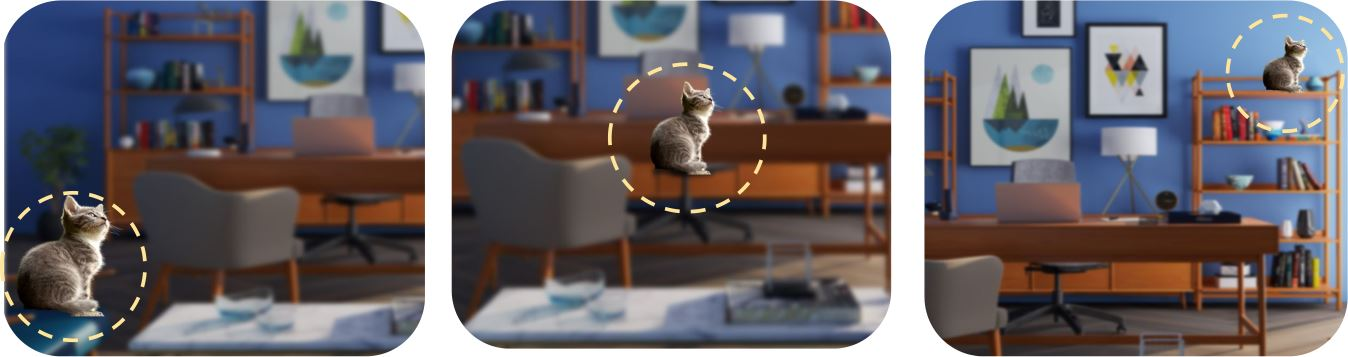
\includegraphics[width=\textwidth-1in]{translationalinvarianceforcnns}
		\caption[Translational invariance for CNNs]{Translational invariance for CNNs.}
		\label{fig:translationalinvarianceforcnns}
	\end{figure}

	\begin{figure}[tbh]
		\centering
		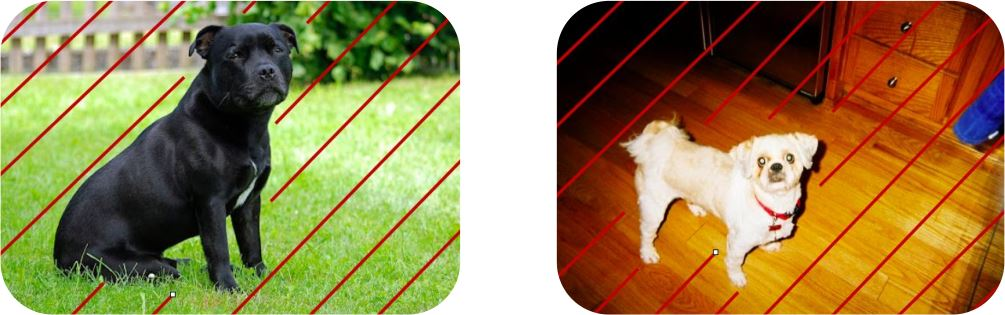
\includegraphics[width=\textwidth-1in]{cnnsignorebackground}
		\caption[CNNs ignore background]{CNNs ignore background.}
		\label{fig:cnnsignorebackground}
	\end{figure}

	\subsection{Computational Advantage of CNNs}
	\begin{bulletedlist}
		\item \textbf{Weight sharing}: In the convolution process, we apply the same filter to every patch of the image.
As a result:
		\begin{bulletedlist}
			\item It reduces the number of weights that must be learned, which reduces training time and cost.
			\item It makes the filter search insensitive to the location of the important features in the image.
		\end{bulletedlist}
		\item Let's say we have an image of size 50x50x3 (i.e.\ 7500 pixels or features) as represented in \figurename~\ref{fig:cnnfeatures}.
		\begin{bulletedlist}
			\item Taking a CNN Layer with 10 filters and a kernel size of 3x3, we'll have the given output of size 48x48x10 size having 23040 features.
			\item Unlike in ANNs, the number of trainable parameters still remains a small fraction of the features and does not scale with that large number.
			\item Number of trainable parameters = (filter size x number of channels + bias) x No. of filters = (3x3x3 + 1) x 10 = 280
		\end{bulletedlist}
	\end{bulletedlist}

	\begin{figure}[tbh]
		\centering
		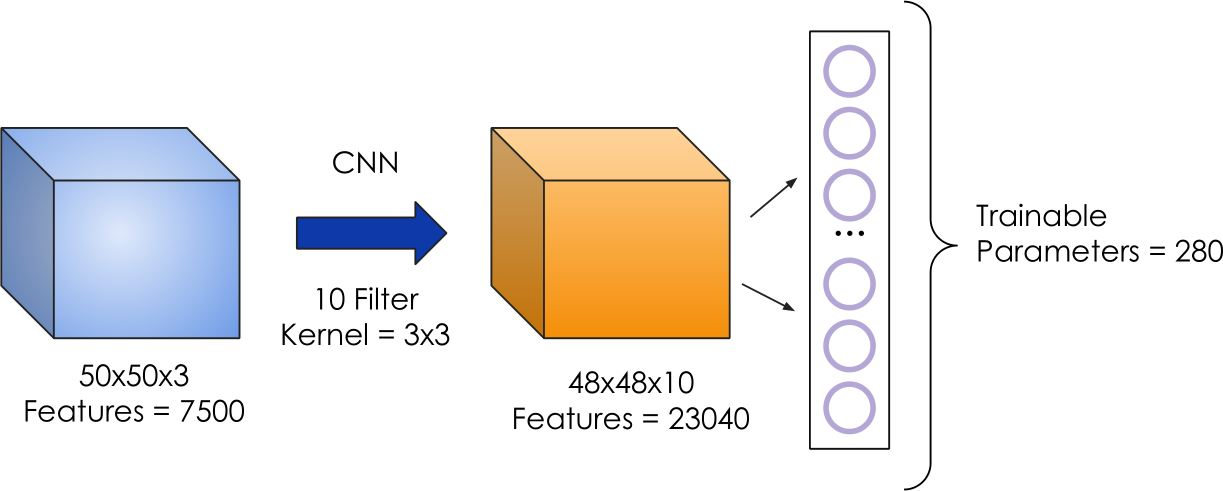
\includegraphics[width=\textwidth-2in]{cnnfeatures}
		\caption[CNNs features]{CNNs features.}
		\label{fig:cnnfeatures}
	\end{figure}

	\subsection{Summary}

	\begin{bulletedlist}
		\item CNNs perform better than ANNs in the crucial task of capturing the relevant features from an image, by ignoring any spatial and translational transformations.
		\item The use of filters in a CNN helps us reduce the dimensionality of the image and extract only the important and required information.
		\item Convolutional filters require exponentially less trainable parameters in comparison to the fully-connected dense layers required in ANNs, and this gives CNNs a computational advantage over ANNs as well.
	\end{bulletedlist}

	\section{CNN Architecture}

	\begin{bulletedlist}
		\item The CNN architecture for image classification is comprised of two major parts:
		\begin{numberedlist}
			\item The feature extraction stage with (a) Convolution layer + Activation function and (b) Pooling layer.
			\item The prediction stage with (a) Flatten layer and (b) Fully connected layer.
		\end{numberedlist}
	\end{bulletedlist}

	\begin{figure}[tbh]
		\centering
		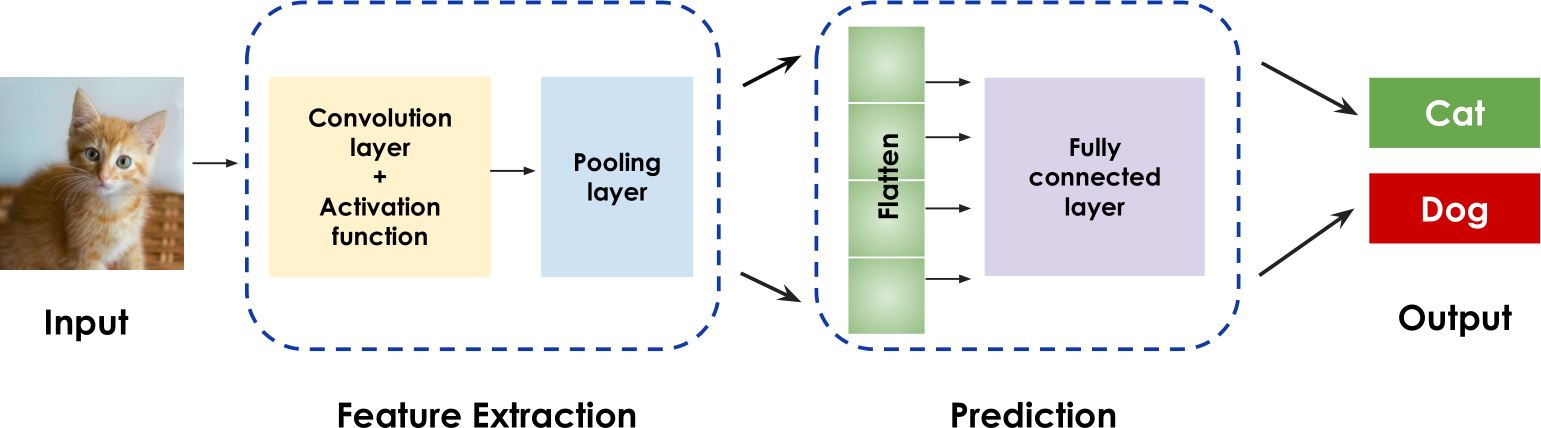
\includegraphics[width=\textwidth-1in]{cnnarchitecture}
		\caption[CNNs architecture]{CNNs architecture.}
		\label{fig:cnnarchitecture}
	\end{figure}

	\subsection{Convolutional Layer}

	\begin{bulletedlist}
		\item In the convolutional layer, a filter is applied on an input image to build a feature map.
		\item Filters can be custom made.  In convolutional neural networks though, the values of the filters are learned through training to determine the important features that can categorize the image more accurately. We simply pass the number of filters and their sizes to the CNN, and the model learns the filter values to develop various feature maps that capture the presence of the features detected.
	\end{bulletedlist}

	\begin{figure}[tbh]
		\centering
		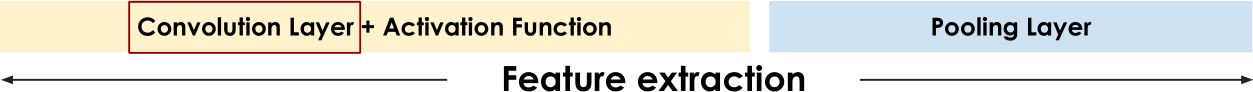
\includegraphics[width=\textwidth-1in]{cnnfeatureextraction}
		\caption[CNN feature extraction]{CNN feature extraction.}
		\label{fig:cnnfeatureextraction}
	\end{figure}

	\begin{figure}[tbh]
		\centering
		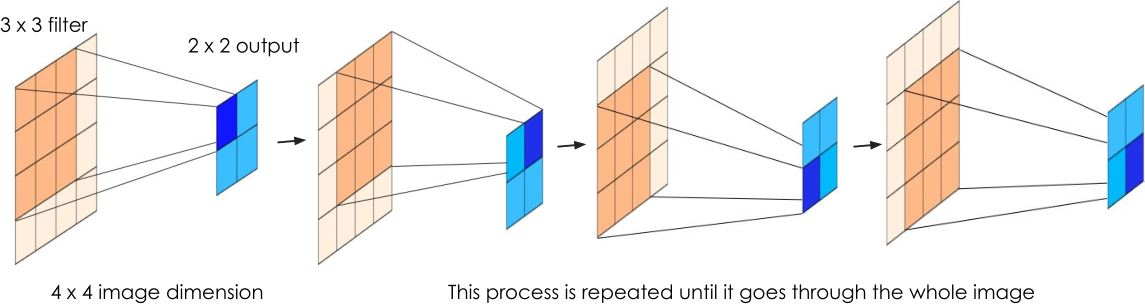
\includegraphics[width=\textwidth-1in]{cnnconvolution}
		\caption[CNN convolution]{CNN convolution.}
		\label{fig:cnnconvolution}
	\end{figure}


	\subsubsection{Activation Function}
	\begin{bulletedlist}
		\item The next step is the Activation Function. In CNNs, the ReLU activation function is used to incorporate a non-linear component into neural networks.
		\item The ReLU function is used in CNNs because the convolution operation is essentially a linear operation (a sum of element-wise products) between the image and the filter, and ReLU adds the non-linearity required for this operation to be able to detect complex non-linear boundaries in the image.
		\item One advantage of using ReLU (Rectified Linear Unit) is that if there are any negative pixels, the function will convert it into zero. This is useful for visualizing these image maps, since negative pixels have no meaning, and it makes subsequent computations more efficient since zeros are easy to work with.
	\end{bulletedlist}

	\begin{figure}[tbh]
		\centering
		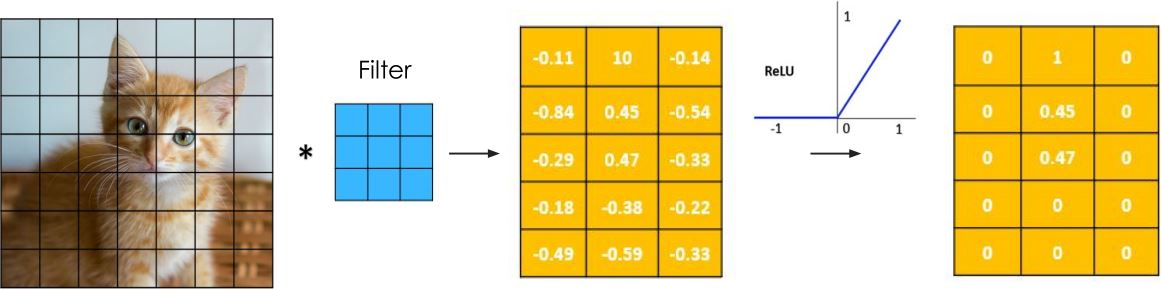
\includegraphics[width=\textwidth-1in]{cnnactivationfunction}
		\caption[CNN activation function]{CNN activation function.}
		\label{fig:cnnactivationfunction}
	\end{figure}


	\subsubsection{Pooling Layer}
	\begin{bulletedlist}
		\item The next step in the Feature Extraction stage is Pooling.  The pooling layer helps in removing unwanted features from the image.  In doing so, it reduces the size of the image and hence decreases the computational cost of the model.
		\item CNNs can use `Max Pooling' (see \figurename~\ref{fig:maxpooling}) to create a pooled feature map using only the maximum values of each patch, and dispose of the unnecessary pixel information.
		\item An important question here is - Do we lose information in this process?  The answer is Yes.  The final feature map includes fewer cells and thus less information than the original input image.  But, the purpose of this step is to discard irrelevant features so that the network can do its job more efficiently.
		\item This process is what's responsible for the ``spatial invariance'' property of CNNs.  Pooling also reduces the size of the images, and hence the number of parameters, which minimizes the likelihood of ``over fitting'', which neural networks are often susceptible to.
	\end{bulletedlist}

	\subsubsection{Flatten Layer}
	\begin{bulletedlist}
		\item After the Feature Extraction stage, we move to the Prediction stage of the CNN.  The first step of the Prediction stage is the Flatten layer.
		\item In this layer, the CNN literally flattens the pooled feature map into a column vector, and the output is used in a standard artificial neural network configuration, which are the fully connected layers of the CNN.
	\end{bulletedlist}

	\begin{figure}[tbh]
		\centering
		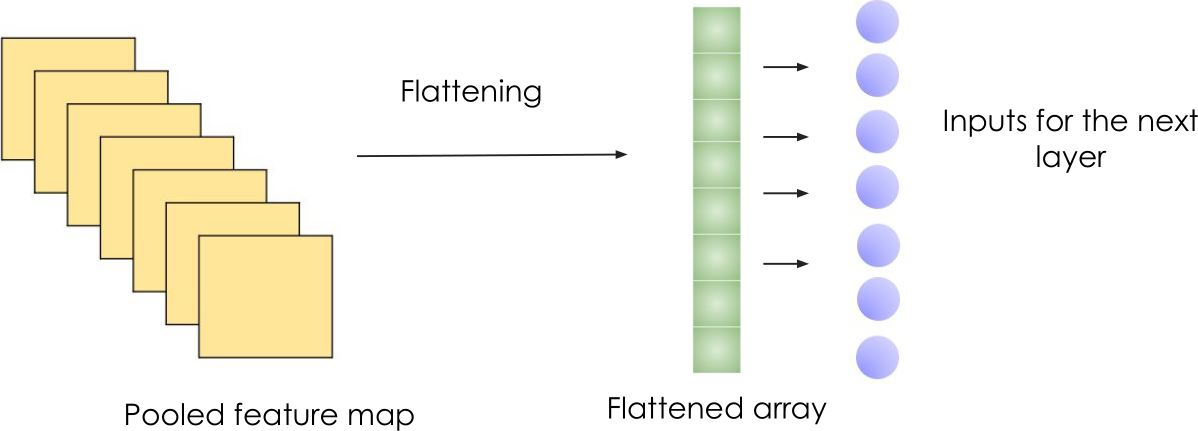
\includegraphics[width=\textwidth-2.0in]{cnnflattenpooledfeaturemap}
		\caption[Flattening pooled features maps to an array]{Flattening pooled features maps to an array.}
		\label{fig:cnnflattenpooledfeaturemap}
	\end{figure}

	\subsubsection{Fully Connected Layer}
	\begin{bulletedlist}
		\item So far, we have learned about the convolution operation, the activation function, pooling and flattening. The final stage of the process is the fully connected layer, where the information from the previous layers is sent to an artificial neural network architecture with Dense (fully connected) layers.
		\item The aim of this step is to take the input and combine the features into a wider variety of attributes that make the convolutional network more capable of categorizing images, which is the sole purpose of building a convolutional neural network.
	\end{bulletedlist}

	\section{Building a CNN Model}
	\begin{bulletedlist}
		\item Let's say we want to build a simple Convolutional Neural Network (CNN) for a prediction problem.  Let's say we need to classify an image as a dog or a cat.
		\item We can build a simple CNN with convolution and pooling layers to solve this problem.
	\end{bulletedlist}

	\begin{figure}[tbh]
		\centering
		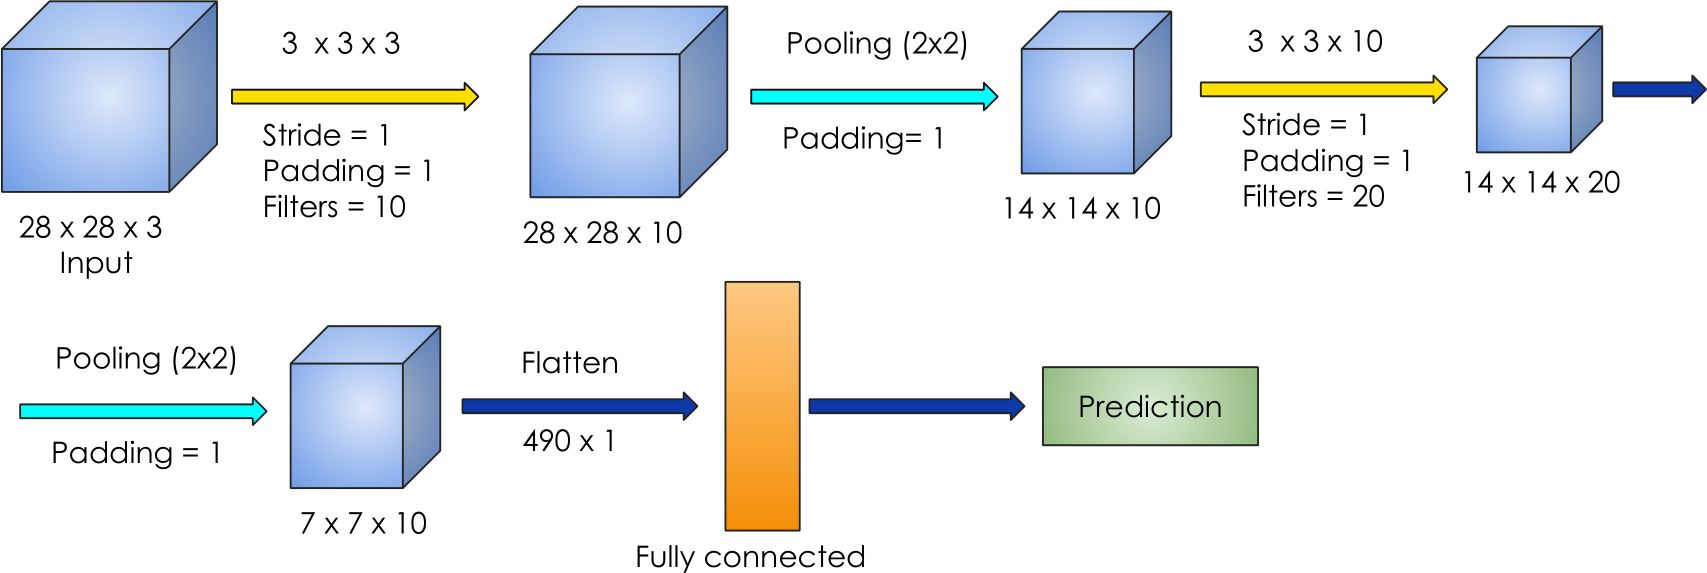
\includegraphics[width=\textwidth-0.75in]{cnnexamplesetup}
		\caption[CNN basic example]{CNN basic example.  The fully connected object is meant to represent one or more hidden layers in a neural network.}
		\label{fig:cnnexamplesetup}
	\end{figure}

	\subsection{Summary}
	\begin{bulletedlist}
		\item We are starting off by applying filters to input images in the form of a convolutional layer.
		\item We break up the linearity of the convolution operation, using the ReLU activation function.
		\item We reduce the image dimension using pooling, for isolating the important features and computational efficiency.
		\item We flatten the feature map and feed it into a fully-connected neural network to generate the final predictions.
		\item Throughout this process, the trainable parameters of the CNN - the weights and filter values, are trained and continuously updated through back propagation so that the CNN can achieve its best possible performance in image prediction tasks.
	\end{bulletedlist}

	\section{Introduction}

Convolution neural networks are a special type of neural network designed to work with image data.  CNNs use convolutional layers hidden layers which perform convolution operations.  They have some different characteristics to artificial neural networks.
	\begin{bulletedlist}
		\item Unlike ANNs, CNNs capture the spatial structure of the image.
		\item CNNs follow the concept of parameter sharing i.e. one filter is applied over the whole image, because of which they are much more computationally efficient.
		\item The first part in this architecture is the convolutional layer followed by the pooling layer and the second part is the fully connected layer.  This whole architecture is called a convolutional neural network.
	\end{bulletedlist}

	\begin{figure}[h]
		\centering
		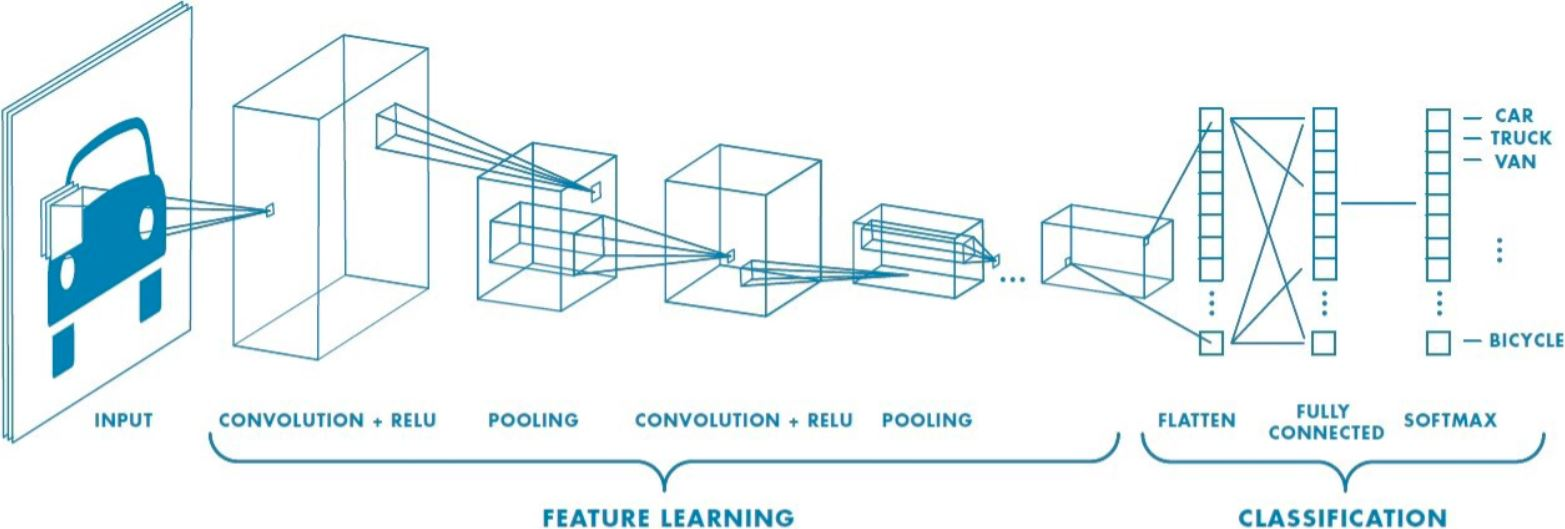
\includegraphics[width=\textwidth-0.5in]{convolutionneuralnetwork}
		\caption[Convolution neural network]{Convolution neural network.  Image source \href{https://towardsdatascience.com/a-comprehensive-guide-to-convolutional-neural-networks-the-eli5-way-3bd2b1164a53}{toward data science}.}
		\label{fig:convolutionneuralnetwork}
	\end{figure}

	\section{Convolutional Layer - Filter/Kernel}
	\begin{bulletedlist}
		\item A convolution operation uses a small array of numbers called a filter/kernel on the input image.
		\item Each filter is designed to identify a specific feature in the input space of the image, such as horizontal edges, vertical edges etc.
		\item A CNN is able to successfully capture the spatial and temporal dependencies in an image through the application of relevant filters.
		\item The role of the CNN is to reduce the images into a form which is easier to process, without losing features which are important for getting a good prediction.
		\item The convolution is performed as shown in \figurename{}s~\ref{fig:convolutionoperationstepsa} and~\ref{fig:convolutionoperationstepsb}.
	\end{bulletedlist}

	\section{Pooling Layer in CNNs}

	\begin{bulletedlist}
		\item After a convolution operation, we usually perform pooling to reduce the dimensions of the feature map.
		\item It enables us to reduce the number of parameters, which both reduces the training time and the over fitting.
		\item Pooling layers down sample each feature map independently, reducing the height and width, but keeping the depth same.
		\item There are two types of pooling - Max and Average.  Max pooling just takes the maximum value whereas average pooling takes the average value in the pooling window (see \figurename~\ref{fig:poolingtypes}).
		\item Contrary to the convolution operation, pooling has no parameters.
	\end{bulletedlist}

	\begin{figure}[h]
		\centering
		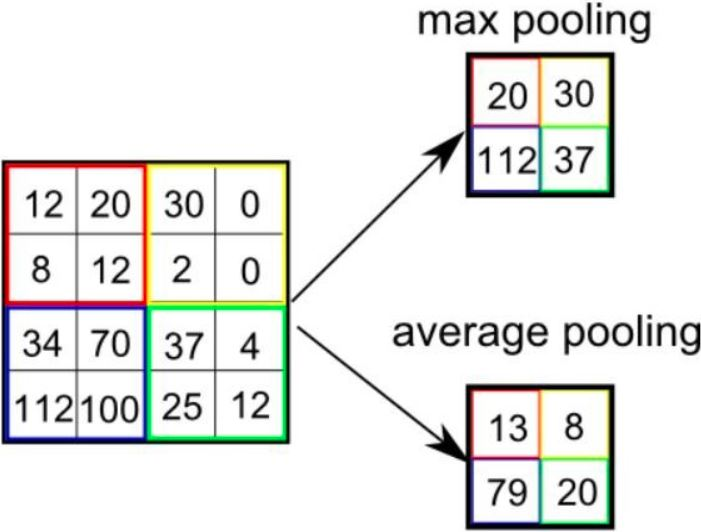
\includegraphics[height=1.5in]{poolingtypes}
		\caption[Types of pooling]{Types of pooling.}
		\label{fig:poolingtypes}
	\end{figure}

	\section{Padding and Stride in CNNs}
	\begin{bulletedlist}
		\item Stride specifies how much we move the filter at each step. By default the value of the stride is 1 and is represented by the first figure
		\item We can also increase the value of stride if we want less overlap between the filters. It also makes the resulting feature map smaller since we are skipping over some locations.
		\item The second figure demonstrates the stride 2.
	\end{bulletedlist}

We see that after using stride, the size of the feature map is smaller than the input. If we want to maintain the same dimensions, we can use padding to surround the input with zeros.  In the following, refer to \figurename~\ref{fig:paddingandstrideincnn}.

	\begin{bulletedlist}
		\item The grey area around the input in the third figure is the padding.
		\item We either pad with zeros or the values on the edge, to match the dimensions of the feature map with the input.
		\item Padding is commonly used in CNNs to preserve the size of the feature maps, otherwise they would shrink at each layer, which is not desirable.
	\end{bulletedlist}

	\begin{figure}[h]
		\centering
		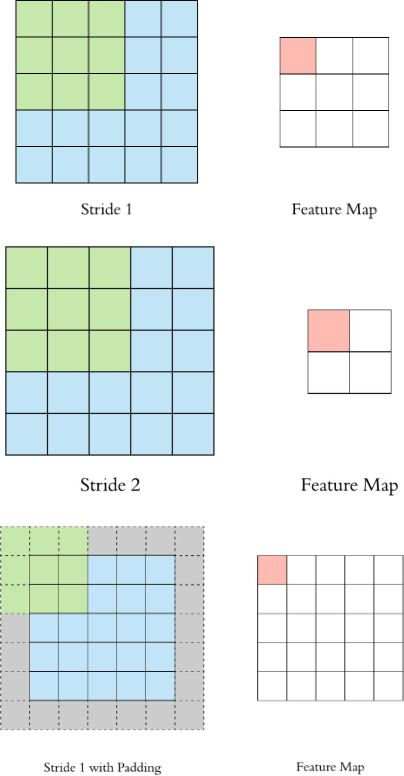
\includegraphics[height=3.5in]{paddingandstrideincnn}
		\caption[Padding and stride in CNNs]{Padding and stride in CNNs.}
		\label{fig:paddingandstrideincnn}
	\end{figure}





	\section{Model Building Practices}
What should the order of different layers in a Convolutional Neural Network be? Where should I put my Batch Norm, Dropout, Activation, and Pooling layers?  Are there any guidelines regarding the same?

	\subsection{Dropout vs Batch Normalization}
The standard deviation issue.

There is a big problem that appears when you mix these layers, especially when Batch Normalization is right after Dropout.
Dropouts try to keep the same mean of the outputs without dropouts, but it does change the standard deviation, which will cause a huge difference in the Batch Normalization between training and validation. (During training, the Batch Normalization receives changed standard deviations, and accumulates and stores them. During validation, the dropouts are turned off, the standard deviation is not a changed one anymore, but the original. But Batch Normalization, because it's invalidation, will not use the batch statistics, but the stored statistics, which will be very different from the batch statistics).

So, the first and most important rule is: don't place a Batch Normalization after a Dropout (or a SpatialDropout).
Usually,  try to leave at least two convolutional/dense layers without any dropout before applying a batch normalization, to avoid this.

	\subsection{Dropout vs Batch Normalization}
If done in an improper order, it can result in changing the zeros to another value.

Also important, the role of the Dropout is to zero the influence of some of the weights of the next layer.  If you apply a normalization after the dropout, you will not have zeros anymore, but a certain value that will be repeated for many units.  And this value will vary from batch to batch. So, although there is noise added, you are not killing units as a pure dropout is supposed to do.

	\subsection{Dropout vs MaxPooling}
The problem of using a regular Dropout before a MaxPooling is that you will zero some pixels, and then the MaxPooling will take the maximum value, sort of ignoring part of your dropout. If your dropout happens to hit a maximum pixel, then the pooling will result in the second maximum, not in zero.
So, Dropout before MaxPooling reduces the effectiveness of the dropout.

	\subsection{Batch Normalization vs Activation}
Depending on the activation function, using a batch normalization before it can be a good advantage.
For a ReLU activation, the normalization makes the model fail-safe against a bad luck case of ``all zeros freeze a ReLU layer.''  It will also tend to guarantee that half of the units will be zero and the other half linear.

For a sigmoid or a tanh, the Batch Normalization will guarantee that the values are within a healthy range, avoiding saturation and vanishing gradients (values that are too far from zero will hit an almost flat region of these functions, causing vanishing gradients).
There are people that say there are other advantages if you do the contrary, I'm not fully aware of these advantages, I like the ones I mentioned very much.

	\subsection{Dropout vs Activation}
With ReLU, there is no difference, it can be proved that the results are exactly the same (Links to an external site.)Links to an external site.

With activations that are not centered, such as sigmoid putting a dropout before the activation will not result in zeros, but in other values.  For a sigmoid, the final results of the dropout before it would be 0.5.

If you add a tanh after a dropout, for instance, you will have the zeros, but the scaling that dropout applies to keep the same mean will be distorted by the tanh.

	\subsection{MaxPooling vs Activation}
There is nothing much here. If the activation is not very weird, the final result would be the same.

	\subsection{Conclusions}
Find the appropriate order of layers which is often useful
	\begin{bulletedlist}
	\item Group 1
		\begin{bulletedlist}
			\item Convolution
			\item Batch Norm
			\item Activation
			\item MaxPooling
			\item Dropout or SpatialDropout
		\end{bulletedlist}
	\item Group 2
		\begin{bulletedlist}
			\item Convolution
			\item ----- (there was a dropout in the last group, no Batch Norm here)
			\item Activation
			\item MaxPooling
			\item Dropout or SpatialDropout (decide to use or not)
			\item After two groups without dropout, can use Batch Norm again
		\end{bulletedlist}
	\end{bulletedlist}